\documentclass{article}
\title{
    \LARGE Agile Working - Project idea\\[0.2em]
    \Large Pineapple Planner
}
\author{Max Sellick, Varvara Aladyina, Deinoras Krasauskas,\\ Azhaf Kahn, Simon Ostini}
\date{February 2025}

\usepackage{graphicx}
\graphicspath{{images/}}

\usepackage{booktabs}

\usepackage{float}
\usepackage[utf8]{inputenc}
\usepackage[english]{babel}
\usepackage[style=ieee]{biblatex}
\addbibresource{references/references.bib}
\usepackage{csquotes}
\usepackage[utf8]{inputenc}
\usepackage{hyperref}
\hypersetup{
    colorlinks=true,
    linkcolor=black,
    filecolor=magenta,
    urlcolor=blue,
}
\usepackage{listings}
\usepackage{multirow, makecell}
\usepackage{pgfplots}
\pgfplotsset{compat=1.18}
\usepackage{caption}
\usepackage{calculator}
\usepackage{calculus}
\usepackage{geometry}
\geometry{
    a4paper,
    left=30mm,
    right=30mm,
    top=25mm,
    bottom=30mm,
    headheight={90pt},
}
\usepackage[shortlabels]{enumitem}

\usepackage{enumitem}
\usepackage{tabularx}
\usepackage{booktabs}

\addto\captionsenglish{\renewcommand{\listfigurename}{Plots}}
\addto\captionsenglish{\renewcommand{\listtablename}{Tables}}

\begin{document}
\begin{figure}[ht!]
  \minipage{0.76\textwidth}
  
\includegraphics[width=7cm]{images/hkr.png}
  \label{title}
  \endminipage
  \minipage{0.32\textwidth}
  \endminipage
\end{figure}

\vspace{0.8cm}
\large

\textbf{{\let\newpage\relax\maketitle}}

\begin{center}
  \vfill
  \small{Kristianstad University | SE-291 88 Kristianstad | +46 44 250 30 00 | www.hkr.se}
\end{center}

\thispagestyle{empty}

\newpage

\makeatletter
\renewcommand{\abstractname}{\vspace{-\baselineskip}}
\begin{abstract}
  \large
  \noindent\textbf{Title}\\
  Agile Working - Project idea\\[1em]
  \textbf{Programme}\\
  Software Development\\[1em]
  \textbf{Authors}\\
  Max Sellick, Varvara Aladyina, Deinoras Krasauskas, Azhaf Khan, Simon Ostini\\[1em]
  % Abstract\\[1em]
  \textbf{Keywords}\\
  Agile, Scrum, Project idea\\[1em]
\end{abstract}
\makeatother

\newpage

\tableofcontents
\thispagestyle{empty}

\newpage

\section{Task 1}

Time management is a challenge for individuals that have multiple responsibilities across work, studies, and personal life, that leads to increased stress and decreased productivity.
Study-related stress and disruption of mental health may take origins from procrastination which is quite common for people with poor time management \cite{ nayak2019impact}.

Traditional calendars and to-do lists, while useful, may not provide the comprehensive support needed to manage these demands effectively \cite{bek2014study}.
For improving individual’s efficiency, to-do list may be implemented calendar for efficiency.

The desktop application “Pineapple Planner” is a task management tool with integrated calendar, to-do list which aims to minimize stress to help completing daily tasks and improves personal productivity.
The app will include recurring tasks, custom task categories, reminders, and priority levels.
Dependencies between tasks will be displayed visually, helping users understand how their tasks relate to one another.

The application is focused on improving mental health stability with focus on SDG 4.3.2 \cite{worldhealthorganisation_2024_sdg}.
Additionally, it aims to contribute to structure people’s lives and to help them achieve their daily goals avoiding task-related stress.

\section{Task 2}
Considering ethical aspects and social responsibility in the development of the Pineapple Planner desktop application is crucial to ensure fairness, accessibility, and user trust.
Ethical principles help create a product that respects user privacy and promotes inclusivity.

One key consideration is data privacy and security.
Task management applications often store sensitive personal information, so implementing strong data protection measures aligns with ethical guidelines such as the General Data Protection Regulation.
Ensuring that user data is stored securely in a Firebase store and not exploited for commercial gain fosters trust and transparency.
\cite{hoofnagle2019european}

Additionally, our application should avoid manipulative design and addictive features that pressure users.
Dark patterns, such as misleading notifications, excessive reminders, or barriers to account deletion, must be eliminated to ensure user control.
Instead, the design should promote productivity without fostering dependency.
To support ethical use, the application should offer customizable notifications, break reminders, and transparent data policies.
Clearly explaining data usage and providing simple consent options will reinforce trust and align with ethical standards.
\cite{montag2019addictive}

Many tools currently being marketed are, intentionally or not, contributing to "hustle" culture, which leads to rapid burnout. 
While making PineapplePlanner we will make sure that our app does as little as possible to lead to immature burnouts.

\newpage

\section{Task 3}
\begin{enumerate}[a)]
  \item We plan to develop the Pineapple Planner app with scalability and usability in mind.
        By using Domain-Driven Design (DDD) with C\verb|#|, WPF, and Blazor, the system will be modular and easy to maintain, allowing the integration of new features over time if required.
        The combination of WPF for desktop and Blazor for web components will ensure a user-friendly and responsive interface.
        Technically, our infrastructure allows easy migration to cross-platform usage.
        With C\verb|#|’s strong type safety and GitHub’s CI/CD pipelines, the app will maintain data integrity and deliver stable updates.
        Lastly, we will strongly profit from JIRA's structured project and task management.
  \item We intend to build a C\verb|#| WPF application that integrates a Blazor web appplication as an external assembly.
        The Blazor app accesses data from a database through queries and commands (CQRS) which are implemented in the application layer assembly.
        The application layer accesses our entities that are defined in the domain layer.
        Generally, it can be said that we plan to use a microservice architecture according to the Domain-Driven-Design (DDD) infrastructure pattern also known as the \textit{Onion architecture}.
\end{enumerate}
\begin{figure}[t!]
  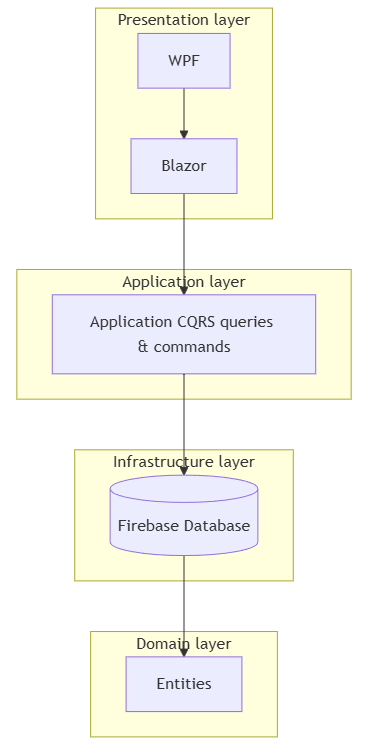
\includegraphics{images/infrastructure-proposal.png}
  \label{Infrastructure proposal}
  \caption{Infrastructure proposal}
\end{figure}
\clearpage

\section{Task 4}

\begin{table}[h]
  \centering
  \begin{tabularx}{\textwidth}{l|X|l}
    \toprule
    \textbf{Nr} & \textbf{Requirement item}                             & \textbf{Priority (High/Medium/Low)} \\
    \hline\hline
    R1          & The user shall be able to inspect their tasks.        & High                                \\
    \hline
    R2          & The user shall be able to manage their tasks.         & High                                \\
    \hline
    R3          & The user shall link their task data to their account. & High                                \\
    \hline
    R4          & The user shall be able to prioritize tasks.           & Medium                              \\
    \hline
    R5          & The user shall be able to set recurring tasks.        & Medium                              \\
    \hline
    R6          & The user shall be able to set reminders for tasks.    & Low                                 \\
    \bottomrule
  \end{tabularx}
  \caption{Requirement items}
  \label{Requirement items}
\end{table}

\begin{table}[h]
  \centering
  \begin{tabularx}{\textwidth}{l|X|l}
    \toprule
    \textbf{Nr} & \textbf{Requirement item}                                                                                                                     & \textbf{Priority (High/Medium/Low)} \\
    \hline\hline
    D1          & Task items are listed in a todo list view and visible in a calendar view.                                                                     & High                                \\
    \hline
    D2          & A task form allows the users to create, edit and delete their tasks.                                                                          & High                                \\
    \hline
    D3          & The application saves a users' tasks in a database.                                                                                           & High                                \\
    \hline
    D4          & Tasks can be assigned priority levels (e.g., High/Medium/Low) with visual indicators (e.g. color-coding) in the todo list and calendar views. & High                                \\
    \hline
    D5          & Tasks can be set to repeat daily, weekly, monthly, or custom intervals.                                                                       & Medium                              \\
    \hline
    D6          & A notification system alerts users via desktop notifications.                                                                                 & Low                                 \\
    \bottomrule
  \end{tabularx}
  \caption{Design items}
  \label{Design items}
\end{table}

\clearpage

\section{Task 5}

\begin{table}[h]
  \centering
  \begin{tabularx}{\textwidth}{l|X|X|X|X}
    \toprule
    \textbf{Sprint}       & Sprint 1                          & Sprint 2                          & Sprint 3                          & Sprint 4                          \\
    \hline\hline
    \textbf{Scrum master} & Varvara\newline Aladyina          & Deinoras Krasauskas               & Azhaf Khan                        & Max Sellick,\newline Simon Ostini \\
    \hline
    \textbf{Developers}   & Max Sellick,\newline Simon Ostini & Varvara\newline Aladyina          & Deinoras Krasauskas               & Azhaf Khan                        \\
    \hline
    \textbf{Tester}       & Deinoras Krasauskas               & Azhaf Khan                        & Max Sellick,\newline Simon Ostini & Varvara\newline Aladyina          \\
    \hline
    \textbf{Support}      & Azhaf Khan                        & Max Sellick,\newline Simon Ostini & Varvara\newline Aladyina          & Deinoras Krasauskas               \\
    \bottomrule
  \end{tabularx}
  \caption{Sprint role planning}
  \label{Sprint role planning}
\end{table}

\clearpage

\section{References}
\printbibliography[heading=none]

\end{document}
